\documentclass{article}
\usepackage[utf8]{inputenc}
\usepackage{graphicx}

%%%%%%%%%%%%%%%%%%%%%%%%%%%%%%%%%%%%%%%%%%%%%
\RequirePackage[pdftex,hidelinks]{hyperref}
% For lists
\usepackage{outlines}
\usepackage[shortlabels]{enumitem}
\usepackage{tabularx}
\usepackage{xcolor}
%%%%%%%%%%%%%%%%%%%%%%%%%%%%%%%%%%%%%%%%%%%%%

\title{Performance evaluation of BERTimbau/GPT-3 based Language Models in solving ENEM}
\author{Desnes Nunes (desnesn@usp.br) e Ricardo Primi (rprimi@mac.com)}
\date{\today}

\begin{document}

\maketitle

\begin{abstract}

This paper focus on examining the potential innovation language models in solving multiple choices high-stakes test \textit{Exame Nacional do Ensino Médio} (ENEM), a multidisciplinary entrance exam widely used on Brazilian universities. Since ENEM questions can involve more than one field of knowledge, i.e., a question may require knowledge of both statistics and biology to be solved, this makes this task very interesting to be tackled by Portuguese Language Models (LMs). We analyzed the data of 916 questions administered in years 2010 to 2017 from ENEM Challenge \url{https://www.ime.usp.br/~ddm/project/enem/}. A number of models were tested based on  BERT embeddings (\textit{Bidirectional Encoder Representations from Transformers}, BERTimbau available in portuguese), finetuned, and GPT3 (\textit{Generative Pre-Training Transformer 3} with few shots and "chain of thought" training regimens. Overall, we found an accuracy score of .77 and an F1 score of .77 for the GPT3 models, which represents a new state of the art for ENEM challenge.

    % The abstract is a short text to let people understand what is the document about.
    % It should give the mains highlights of the documents.
    % This document is a template to be use in the Final Project of the EA376E class.
    % The recommendation is to use LaTeX by the application Overleaf.com, but it is also
    % possible to use Google Docs or MS-Word.
\end{abstract}

\section{Introduction}

Needless to say, recent innovations presented not only on LMs applications, but also to whole field of Machine Learning (ML) have been astonishing and seem to have an  almost unlimited application scope. This of course correlates strongly to digital aspects present of modern life; such as banking, chat bots, meal ordering, music listening, meeting people, among many other services. These applications rely heavily on ML processing of customer's data, in order to make Artificial Inteligence (AI) models able provide automatic suggestions, take decisions and more. Moreover, an area that started to receive some attention recently from ML applications is education; which recently saw, for instance, works aiming LMs usage in classrooms \cite{kuvcak2018machine}, as well as the so called \textit{precision education} \cite{luan2021review}. 

On this context, this paper explores the field of Q\&A tackling enhancements of Portuguese trained LMs, in particular, with the usage of state-of-the-art transformer-based models \cite{VaswaniAttentionAllYou2017a} such as BERT \cite{devlin2018bert} and GPT-3 \cite{https://doi.org/10.48550/arxiv.2005.14165}. These models were used here on a series of experiments to answer multiple choice questions from the multidisciplinary \textit{Exame Nacional do Ensino Médio} (\href{https://www.gov.br/inep/pt-br/areas-de-atuacao/avaliacao-e-exames-educacionais/enem}{\underline{ENEM}}), which is an important Brazilian university entrance exam used nationwide. 

The proposed research aims to advance the benchmarks for automatically solving college entrance exam by exploring recent state of the art language models for enhancing the performance of AI on this task answering the call \textbf{ENEM Challenge}  \url{https://www.ime.usp.br/~ddm/project/enem/}. ENEM's purely textual multiple-choice questions pose a challenging problem, requiring advanced natural language processing skills. The problem has been examined in earlier research \cite{8575587} using static word embeddings and WordNet but with limited success attaining an accuracy of 26\% to 29\% of correct responses. Hence, since the dataset of this work has been gratefully made openly available through the \href{https://www.ime.usp.br/~ddm/project/enem/}{\underline{ENEM Challenge}}, this paper proposes to tackle this task with the use of contextual embedding of BERTimbau and the few-shot capabilities of GPT3, since our main hypothesis is that these models can outperform previous studies. By doing so, we aim to improve the accuracy of our model and demonstrate the potential of AI to assist in the education process. The study is important in demonstrating the potential of AI to be used in educational tests, as well as to assess the accuracy and reliability of AI-based solutions. 


%ENEM's purely textual multiple-choice questions pose a challenging problem, requiring advanced natural language processing skills. By doing so, we aim to improve the accuracy of our model and demonstrate the potential of AI to assist in the education process. The study is important in demonstrating the potential of AI to be used in educational tests, as well as to assess the accuracy and reliability of AI-based solutions. 
% The proposed research aims to advance the benchmarks for automatically solving college entrance exam by exploring recent state of the art language models for enhancing the performance of AI on this task answering the call 
%The problem we aim to address is whether these models, which have achieved impressive results on a variety of natural language processing tasks, can also perform well on a standardized educational exam. Our main hypothesis is that BERT and GPT-3 will be able to accurately answer a significant number of ENEM questions, demonstrating their potential to assist in the education process.
%This is an example of paper citation: BERT~\cite{devlin2018bert} is a transformer. T5~\cite{raffel2019exploring} also uses transformers.

\section{Methodology}

\subsection{Data set}

The \href{https://www.ime.usp.br/~ddm/project/enem/ENEMdataset.zip}{\underline{dataset}} published by \cite{DBLP:journals/corr/abs-2201-11903} provides of of its data in xml format, which has been derived from parsing real questions and alternatives that were presented on the ENEM over a few years. Moreover, the authors have labeled each question with the following knowledge tags:

\vspace{-0.15cm}
\begin{itemize}%[leftmargin=*]
  \item Text Comprehension (TC)
  \vspace{-0.25cm}
  \item Encyclopedic Knowledge (EK)
  \vspace{-0.25cm}
  \item Image Comprehension (IC)
  \vspace{-0.25cm}
  \item Domain Specific Knowledge (DS)
  \vspace{-0.25cm}
  \item Mathematical Reasoning (MR)
\end{itemize}
\vspace{-0.05cm}

These tags have been extremely helpful since they inform if a question has an image or mention chemical elements that can't be treated as text. The entire dataset consists of 1754 items from the ENEM language and human sciences tests from 2010 to 2017. After eliminating questions that require understanding of images (IC), reading of symbols of chemical elements (CE) and mathematical reasoning (MR), the final database used here is made of 916 questions. Each item is composed of a \textbf{header} where the main text of the item is presented; a \textbf{statement} where the question is asked to the students and \textbf{alternatives}, containing five options from which one correctly answer the question (statement).

For the fine tuning experiment with BERTimbau we split items randomly into a training set (733 questions) and a test set (183 questions). Three items were selected to create prompts and chain of thought reasoning expected for the solution to use in the few-shot experiments. 

\subsection{Transformer Models}

The models used on this work (BERT and GPT3) are based on the attention mechanism of the transformers architecture which is illustrated on Figure 1.

\begin{figure}[h!]
    \centering
    %\captionsetup{justification=centering}
    \caption{Illustration of BERT and GPU models architecture}
    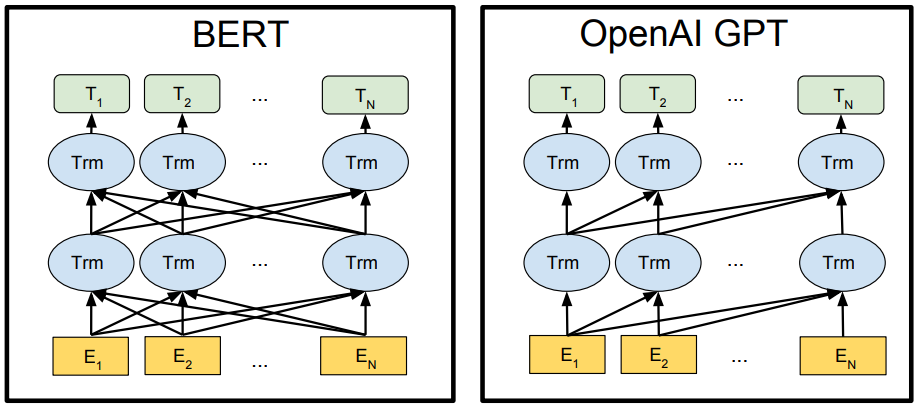
\includegraphics[width=0.75\columnwidth]{figures/4.png}
    \label{fig:3}
    \\
    \text{Source: \cite{https://doi.org/10.48550/arxiv.1907.05338}}
\end{figure}

The core mechanism of transformer's encoder and decoder is called \textit{attention}. Upon receiving tokens in continuous distributed representations (\textit{embeddings}), the encoder adds a representation of the token's position within the sequence. After that, a covariance matrix is calculated between all the vectors of the tokens (illustrated as ellipses in the Figure 1). This matrix stores how similar a token \textit{t} called \textit{query} is to a context called \textit{keys} (including itself). Afterwards, this matrix is converted into weights, called \textit{attention scores}, which range from 0 to 1 after going through a softmax function. With the use of these weights, a new representation of each token called \textit{value} is computed based on a weighted average of the embeddings of all tokens in the sequence. Thus, if the vectors of two tokens are eventually more similar, they will be recalculated by a weighted average of both. As opposed to this, if two tokens have zero correlation, they will remain unchanged. The transformation of the original vectors of each token enables the recreation of the vectors based on the similarity with those of the context tokens, thus enabling contextual representations - and this is the core attention mechanisms \cite{peltarion22}.

These representations are more powerful than the static word embeddings \cite{MikolovEfficientEstimationWord2013a} used by the previous work \cite{8575587} which tackled portuguese Q\&A for ENEM question solving; therefore, we expect improved performance with the use of models which rely heavily on the attention mechanism, such as BERT and GPT-3.

Also, one important aspect related to GPT3 that has been started to be tackled here is the enhancement of few-shots prompts techniques with CoT \cite{DBLP:journals/corr/abs-2201-11903}. By adding to the prompts a series of intermediate reasoning steps, it is reasonable to believe that this would allow the model to break down complex problems into smaller, more manageable steps, in order to reason each step individually before compiling the results that derive the final answer. In this way, the model can potentially grasp abstract concepts inasmuch manipulate them, in order to solve problems that require deep understanding of underlying principles. This technique may improve large language models' ability to perform complex reasoning. A future work that started to be created here questions whether the usage of CoT in large LMs would enhance their ability to perform complex reasoning tasks, like answering ENEM questions, making them more effective in a variety of applications.

\subsection{Design and models}

This work made use use of four different approaches, which are more thoroughly explained hereafter.

\subsubsection{\textbf{BERtimbau embeddings}}

With the use of \cite{souza2020bertimbau}, the first experiment performed a forward pass for each ENEM item component (header, statement, and five alternatives), saving layer 12 embeddings  for each component. An overall embedding was created by averaging each token embedding that makes up each component. Afterwards, it was calculated the cosine similarity between each header/statement and alternative, and then selected the one with the highest similarity as the correct alternative. In addition, the embeddings of the [CLS] special tokens were saved in order to enable the algorithm to select the alternative whose embeddings were most similar to the embeddings of the [CLS] question.

\subsubsection{\textbf{BERtimbau fine tuning}}

Here five examples were created for each item by concatenating the question's header, statement, and alternatives. The special [SEP] token between the header/statement and the alternative text was also specified. Therefore, in the BERT model, the first segment consists of the header/statement text and the second segment consists of the alternative text. Each example had a target label of 1 if it was paired with the correct alternative and 0 otherwise. Hence, there are five instances of headers/statements with one alternative for each, which creates an unbalanced set of examples, since only 20\% will be correct and 80\% will be incorrect. Due to these circumstances, the correct examples were over-sampled by repeating them four times on the training set. This model was started with pre-trained BERTimbau weights, which latter was trained on the test set for 3 epochs, with learning rate set on $lr = 5e-05$.

\subsubsection{\textbf{GPT3 with 0-shot / few shot}}

By utilizing the so called 0-shot learning strategy on GPT-3, an algorithm was developed to input and analyze multiple queries into the model; which contained the ENEM question and its alternatives. The model was found to perform better which this setup. Latter, the few-shots was assembled to make the model also receive three different examples, with all alternatives and correct answer before before the question that was being asked.

Token generation was not requested from the model. Rather, it was analyzed the likelihood of each token among the alternatives. By aggregating the log probabilities of each token that comprises the alternative, we calculate the probability of each alternative as follows: 

%\vspace{-0.75cm}
\begin{equation} \label{eq1}
%\begin{split}
probability(alternative_{a}) = e^{\left(\sum_{i}^{N} logprobs[i]/N\right)}
%\end{split}
\end{equation}
where \textit{a} is the alternative - 1 to 5, \textit{i} is the logprob of a token and \textit{N} is the total number of tokens

Moreover, the following parameters on the GPT3 API were used: item temperature = 0, max\_tokens = 1, top\_p = 1, frequency\_penalty=0, presence\_penalty=0, echo=True and logprobs=5.

\subsubsection{\textbf{GPT3 with chain of thought}}

In this model, the only difference from the previous one is that the prompt contained an explanation of why the correct alternative was selected. After that, the model was asked to generate the correct alternative and explanations.

% \begin{figure}[h!]
%     \centering
%     \captionsetup{justification=centering}
%         \caption{Illustration of a N-BERT model and its sesame street mascot}
%     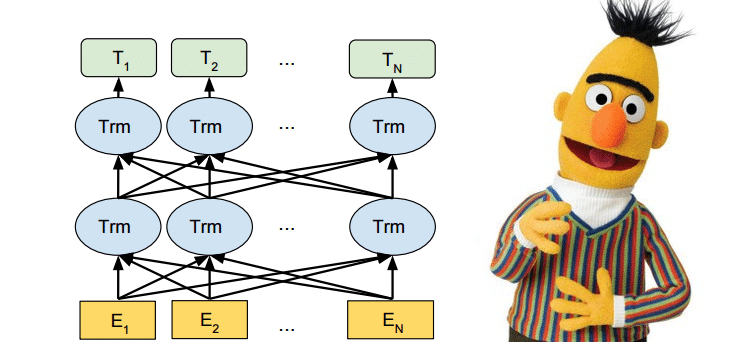
\includegraphics[width=1.0\columnwidth]{Images/3.png}
%     \label{fig:3}
%     \\
%     \text{\footnotesize Source:\cite{morris2019}}
% \end{figure}

% \begin{figure}[ht]
% \centering
% 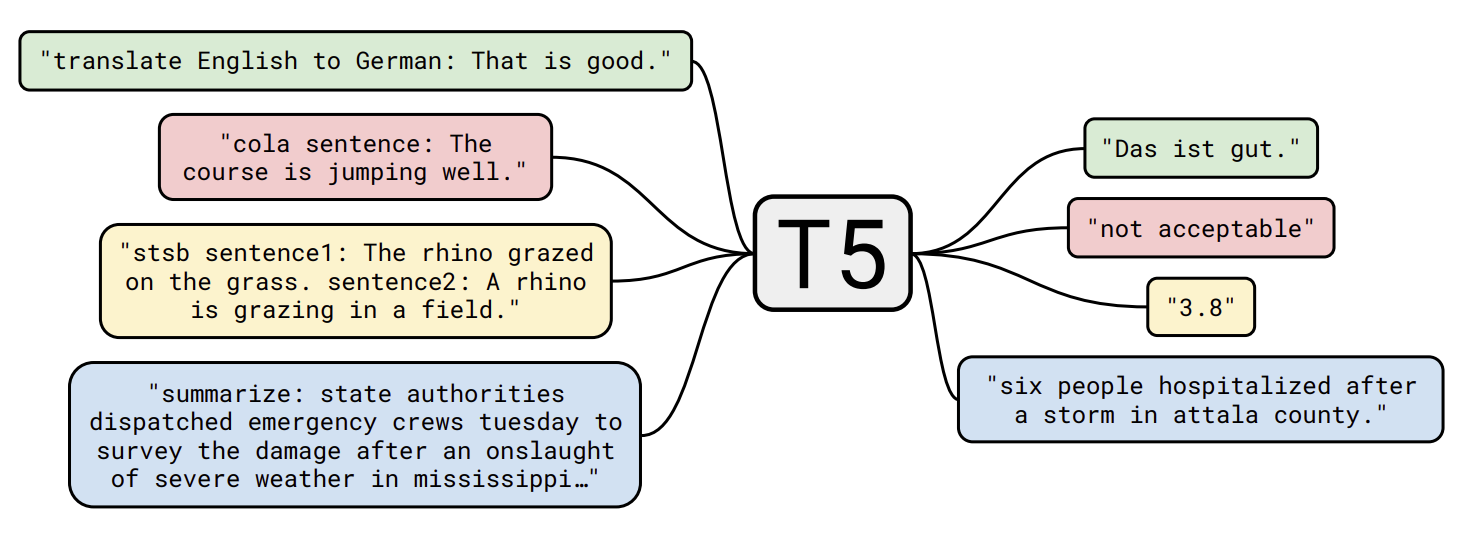
\includegraphics[width=.77\textwidth]{figures/t5.png}
% \caption{\label{fig:t5}Figure example.}
% \end{figure}

% Figure~\ref{fig:t5} is an example of figure citation.
%{\color{red}TODO: Describe XML}

\section{Experiments}

\subsection{Metrics}

The global performance of a model should be evaluated with the use of a global accuracy score and the F1 score by combining \textbf{precision} (the proportion of true correct alternatives out of true positives plus false positives) and \textbf{recall} (the proportion of true correct alternatives out of all correct alternatives, that is, true positives divided by true positives plus false negatives) into one metric by taking their harmonic mean. A few experiments here were able to outperform global accuracy way above 29\%, which was the baseline (reported in \cite{8575587}) for this work.

\subsection{Results}

The experiments using the methodology described above were developed in python and R language. Code and data are available the following github \href{https://github.com/rprimi/enem_challenge}{\underline{repository}}. Futhermore, Table 1 present the main results of our evaluation of the experiments.

%\vspace{-0.05cm}
%\begin{itemize}%[leftmargin=*]
%  \item temperature = 0
%  \vspace{-0.25cm}
%  \item max\_tokens = 1
%  \vspace{-0.25cm}
%  \item top\_p = 1
%  \vspace{-0.25cm}
%  \item frequency\_penalty=0
%  \vspace{-0.25cm}
%  \item presence\_penalty=0
%  \vspace{-0.25cm}
%  \item echo=True
%  \vspace{-0.25cm}
%  \item logprobs=5
%\end{itemize}
%\vspace{-0.05cm}

% \begin{table}[h!]
%     % \centering
%     \caption{Tabela simples}
%     \begin{tabularx}{ l l }
%     \hline
%         cell1 & cell2\\   \hline
%         cell4 & cell5\\    \hline
%         cell7 & cell8\\    \hline
%     \end{tabularx}
%     \\
%     \vspace{0.25cm}
%     \text{\footnotesize Source: Own authorship, 2022.}
%     \label{ta:tabela1}
% \end{table}

%\begin{center}
%\begin{tabular}{|| l c ||} 
% \hline
% \ \ \ \ \ \ \ \ \ \ \ \ \ \ Model & Accuracy \\ [0.5ex] 
% \hline\hline
% text-davinci-002 0-shot no CoT & 77.29\% \\ 
% \hline
% text-davinci-003 0-shot no CoT & B\% \\ 
% \hline
% text-davinci-002 few-shots no CoT & C\% \\ 
% \hline
% text-davinci-002 few-shots with CoT & D\% \\
% \hline
% text-davinci-003 few-shots no CoT & E\% \\
% \hline
% text-davinci-003 few-shots with CoT & F\% \\
% \hline
%\end{tabular}
%\end{center}

\begin{center}
\caption{Table 1 - Results of the four models on solving ENEM questions}
\begin{tabular}{ | l | l | l | }
\hline
	\  & \  & \  \\ \hline
	\textbf{Model} & \textbf{Accuracy} & \textbf{F1} \\ \hline
	  BERTIMbau Embeddings  \\ \hline
	     Heading & 20\% & 0.19 \\ \hline
	     Statement & 21\% & 0.21 \\ \hline
	     [CLS] & 20\% & 0.19 \\ \hline
	\  & \  & \  \\ \hline
	  BERTIMbau Finetuned & 57\% & 0.41 \\ \hline
	\  & \  & \  \\ \hline
	  GPT3 & \  & \  \\ \hline
	    0-shot with davinci-002 & 77\% & 0.77 \\ \hline
	    0-shot with davinci-003 & 77\% & 0.77 \\ \hline
	    % few-shot  davinci-002 & Not completed & Not completed \\ \hline
	    % few-shot  davinci-003 & Not completed & Not completed \\ \hline
	    CoT with davinci-002 & Not completed & Not completed \\ \hline
	    CoT with davinci-003 & Not completed & Not completed \\ \hline
\end{tabular}
\end{center}

\subsection{Issues}

A few issues that didn't allow us to complete all the experiments in all models in the time frame of the assignment are as follows:

\vspace{-0.05cm}
\begin{itemize}%[leftmargin=*]
 \item Most issues of the code arose with parsing the results from the OpenAI model, specially when dealing with multiple shots on GPT-3. On the reply of the model, getting the right position of the tokens of the alternatives in order to also get the position of the logprobs was very tricky. Furthermore, on the CoT experiments the model's reply hanged from time to time (sometimes the model generated an alternative, other times just a latter not properly closed with the \\n string terminator).
 \vspace{-0.25cm}
 \item The CoT examples that were presented to the few-shots model need more investigation. Instead of the same example for all areas, maybe relate them to the type of question that is being answered?
\end{itemize}
\vspace{-0.35cm}

The authors plan to address these issues in future works.

\section{Conclusion}

%Since questions can involve more than one field of knowledge, i.e., a question may require knowledge of statistics and biology to be solved, this makes this Q\&A task very interesting to be tackled by portuguese Language Models (LMs). Furthermore, with the usage of \textit{Bidirectional Encoder Representations from Transformers} (BERT) and \textit{Generative Pre-Training Transformer 3} (GPT-3), the results reached here have outperformed previous works by achieving {\color{red}X\%} of accuracy with the usage of {\color{red}davinci-003?} in our best scenario, as shown hereafter.

This paper researched enhancements on the field of Q\&A in Portuguese-BR with the usage of state-of-the-art AI models. With the use of the pre-trained BERT and GPT-3 models, this work was able to reach significant results on answering multiple choices questions from the ENEM, a widely multidisciplinary test used for brazilian universities acceptance.

This research is relevant for several reasons. First, it provides a novel use of BERT and GPT-3 in the educational domain, highlighting their potential in guiding future developments in the use of AI in education. It can be easily assumed that what is being proposed here can serve as a beacon for educational applications such as automatic scoring of achievement tests, automatic writing feedback for assessments, and the adoption of AI-powered tools to assist educators in developing adaptive tests and adaptive learning programs. Second, the findings of this research could also have significant consequences for the education sector, potentially leading to the adoption of AI-powered tools for psychometric analysis of ENEM exams, including predicting the difficulty of questions, developing new items, and ultimately assisting in the creation of adaptive ENEM test-suites. Last, but certainly not least, it also contributes to the growing body of research that attempts to understand the intelligence underlying the language models. Are they capable of understanding? Can they justify their answers by providing human-like explanations of their reasoning that humans consider intelligent?

\section{Future Work}

For starters, future work would certainly involve the conclusion of the experiments with BERTIMbau and few-shots with CoT. Furthermore, an idea brainstormed during this work would involve research on the development of questions within a certain knowledge base, which seems fair to assumed that might have good results with the usage of the GPT-3 and T5 models, for instance.

% Usando a bibliografia com arquivo no formato bibtex, (ver arquivo main.bib que faz parte desse projeto)
\bibliographystyle{plain}
\bibliography{main.bib}

\end{document}
